In Section~\ref{sec:Linear Classifiers}, only very basic linear methods for classification were discussed. The log odds were modeled in a linear fashion and a decision boundary was drawn based on this. In this section the framework is completely different. The linearity assumptions are removed and the multiclass case is considered immediately. 
First, classification trees will be discussed. When this framework is clear, ensemble methods, that try to improve the trees performance, will be presented and discussed. This chapter is the main part of the projecte, and will focus on variations of boosting methods, bagging and random forest. 
%
\section{Classification trees}
\label{sub:Classification trees}
%%fakesubsection Classification trees
A classification tree makes local decisions based on a subset of the predictors. This means that the data is split in subsets, that are again split in new subsets (independently of each other) and so on. 
At the end the subsets are given a class label based on some vote-measure between the data points (usually the majority).
\todo{Always majority?}
And example of such a tree can be found in Figure~\ref{fig:cart}.
The simplicity of the rules makes the method very general, both in terms of nonlinearity and in type of predictors. The method works with continuous, discrete ordered, and categorical predictors. Another benefit is that the resulting tree is highly interpretable, as the splits are easy to visualize. Prediction is done by following splits down to the decision node, giving the predicted class. An example of such a tree can be found in Figure~\ref{fig:cartTree1}.\\
\\
There are several different algorithms using this framework. They differ in the way they are grown, and on the size of the tree.
Unlike the linear classifiers, the decision boundaries can take different forms. Everything from a linear boundary with two end nodes, to a highly complex boundary with the same amount of end nodes as data points is possible. In this regard, the terms \textit{overfitting} and \textit{underfitting} need to be introduced. 

An underfitted model is to simple to capture the complexity of the data. On the contrary, an overfitted model is fitted to close to the training data and therefore describes the random noise of the training data rather than the true underlying model.  Obviously, a full tree, i.e. only one training point in each end node, will be overfitted, while a too small thee will underfitted. 

\todo{Should regression be presented like this?}
In the regression framework, under squared error loss, it can be shown that a small tree is highly biased with low variance, while a larger tree is highly unstable (high variance), but with smaller bias. 
In appendix~\ref{sec:EPE}, it is shown how the $\mathrm{EPE}$, introduced in \ref{sub:LDA and Fisher's linear discriminant}, has an additive relationship with the classifier's bias and variance. Therefore this \textit{bias-variance tradeoff} is important to consider when creating the prediction method. 

For classification the same argument does not quite hold, but similar definitions for bias and variance has been proposed for $0/1$ loss in the literature. Among the most famous are \cite{kong1995error}, \cite{kohavi1996bias}, \cite{breiman1996bias} and \cite{Friedman1997bias}. While they have all provided useful insight to classification problems, non of them present a framework as simple and satisfactory as for regression. In this paper when referring to bias or variance of classifiers, it is more in a heuristic way. Loosely, bias measures the systematic error of a classifier, i.e. the average error over different training sets. Variance measures the additional error do to variations in the classifier between training sets. 
\\
\\
This bias-variance tradeoff is important to consider, and there are different methods created to optimize it.
Some of the more common methods are ID3 by \cite{ID3}, C4.5 by \cite{C4.5} and its successor See5/C5.0, CHAID by \cite{CHAID} and CART by \cite{breiman}.
In this project only CART will be covered, as this might be the most famous of them.
\\ \colorbox{yellow}{Give references to other tree methods than CART.}
\\\url{http://stackoverflow.com/questions/9979461/different-decision-tree-algorithms-with-comparison-of-complexity-or-performance}
%
\subsection{CART}
\label{subsub:CART}
<<cartSim, echo=FALSE>>=
# Simple simulation to get nice areas and tree
source("../code/cartSim.R")
@
\colorbox{yellow}{In this section use both \cite{bishop} , \cite{modstat} and \cite{breiman}.}\\
\url{http://edoc.hu-berlin.de/master/timofeev-roman-2004-12-20/PDF/timofeev.pdf}\\\\
%
The Classification and Regression Trees algorithm split at only \textit{one} variable at the time, i.e. no combinations of features are used in the splits. This means that the domain is split into rectangles, aligned with the axes. 
Also, each split in CART divide the domain in \textit{two} parts, often referred to as binary splitting. Thus, the splits are done in the simplest way possible, but has still shown some decent performance. CART, as the name implies, can be used both for classification and regression, but only its abilities as a classifier will be considered in this section. The regression framework will be briefly introduced in \ref{sub:Gradient boosting}.

In Figure~\ref{fig:cart} a toy example was simulated to illustrate how the CART algorithm works. The tree is made by the R function \verb+rpart+ \cite{rpart}. To make it easy to visualize, only two predictors were used. 
In Figure~\ref{fig:cartAreas1} the domains created by the splits are displayed. Each vertical and horizontal line shows a split. It is clear that the data is not linear, and the figure shows how easy the algorithm handles this.
For more than two predictors it is hard to visualize the splits on the actual domain, so a tree view is used instead.
 In Figure~\ref{fig:cartTree1} the tree from the toy example is displayed. It is clear that it easily generalize to more than two dimensions. \\
%
\begin{figure}[h!]
  \centering
  \begin{subfigure}[b]{0.48\textwidth}
    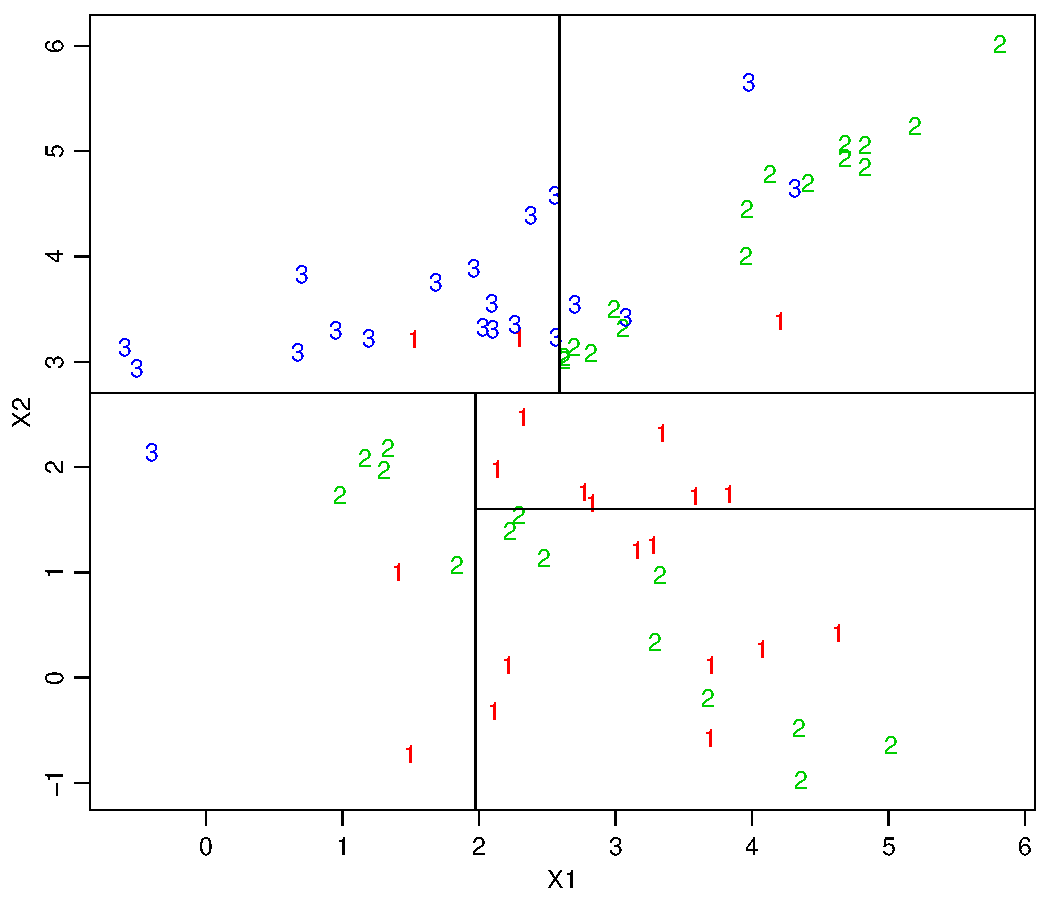
\includegraphics[width=\textwidth]{./figures/cartAreas1.pdf}
    \caption{Decisions displayed as boxes.}
    \label{fig:cartAreas1}
  \end{subfigure}%
  \quad
  \begin{subfigure}[b]{0.48\textwidth}
    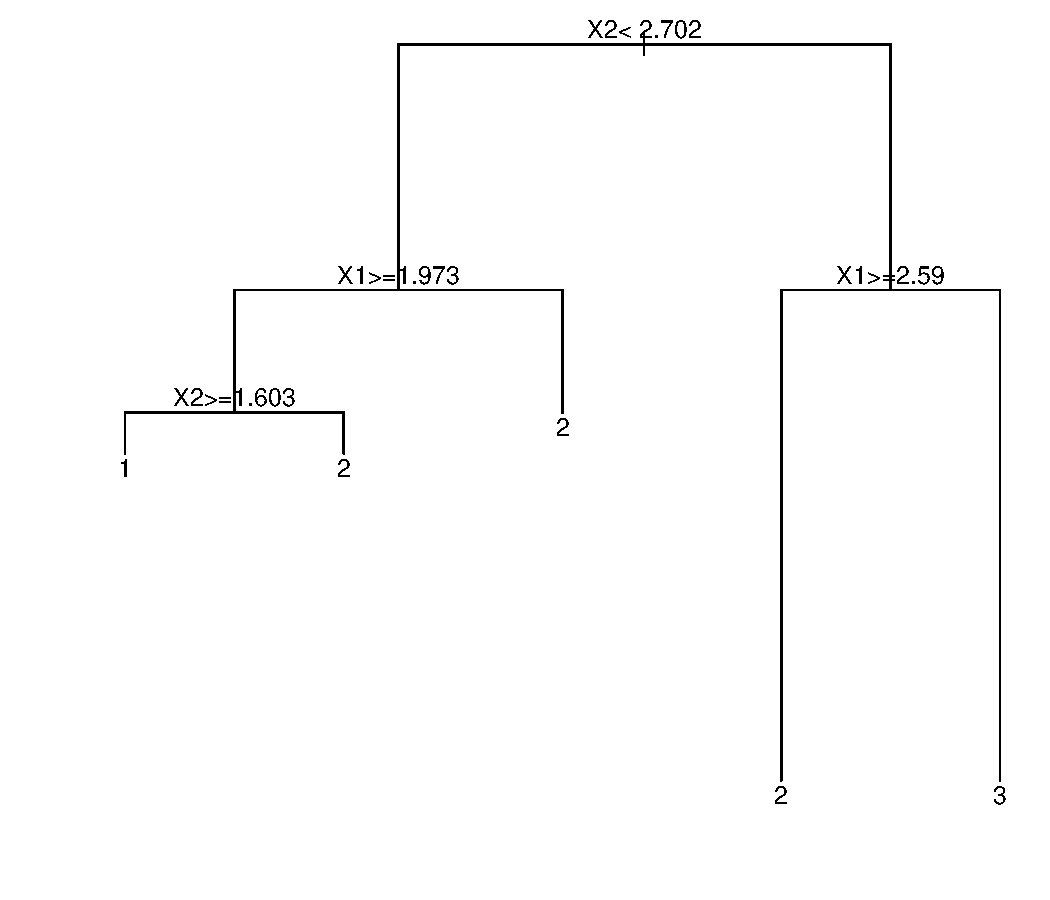
\includegraphics[width=\textwidth]{./figures/cartTree1.pdf}
    \caption{Decisions displayed as a tree.}
    \label{fig:cartTree1}
  \end{subfigure}
          %(or a blank line to force the subfigure onto a new line)
  \vspace{1\baselineskip}
  \caption{CART run on simulated data in two dimensions. }
  \label{fig:cart}
\end{figure}
%
\subsubsection{Growing a tree}
\label{sub:Growing a tree}

The intuition behind CART is pretty straight forward, so what remains is how to grow the tree and how large the tree should be grown. As it is too computationally extensive to create an optimal tree, greedy algorithms for splitting in a sequential matter are used instead. A split needs to to be based on a criterion and one of the more common is the \textit{Gini index}. For $K$ classes it is defined as,
\begin{align}
  Q_m(T) &= \sum^{K}_{k=1} \hat{p}_{mk} (1 - \hat{p}_{mk}),  \\ 
  \label{eq:pmk} 
  \text{where}& \quad \hat{p}_{mk} = \frac{1}{N_m} \sum_{\mathbf{x}_i \in R_m} I\{y_i = k\}.
\end{align}
Here $T$ is the tree, $m$ is a node, $N_m$ is the number of data points in node $m$, $y_i$ is the class of training point $i$ and $R_m$ is the region defined by the node.
$\hat{p}_{mk}$ is therefore the proportion of class $k$ in node $m$.
The Gini index increase with the diversity in the node, and gives therefore a measure of \textit{node impurity}. For nodes with only one class it is zero, and for homogeneous nodes (equal amounts of all classes) it gets its maximum value. The greedy algorithm used by CART finds the split that gives the lowest total node impurity, and weight the two nodes by their size.  
The length of the branches in Figure~\ref{fig:cartTree1} is a representation of the improvement in the node impurity. The longer the branch the higher the gain.

Now, consider the case where a split is performed on node $P$. By splitting on the variable $x_j$, let $R_L(j,s) = \{\mathbf{x} | x_j \leq s\}$ denote the region of the "left" split,  and $R_R(j,s) = \{\mathbf{x} | x_j > s\}$ denote the "right". To find the variable $x_j$ and split point $s$ that gives the lowest node impurity, one solve
\begin{align}
  \min_{j,s} \left\{ \frac{N_L}{N_P} Q_L(T)
  + \frac{N_R}{N_P} Q_R(T) \right\}.
\end{align}
Here $j$ and $s$ lies in $\hat{p}_{mk}$ in \eqref{eq:pmk}. $N_L$, $N_R$ and $N_P$ are the number of observations in the left, right and parent node respectively.
\todo{interpret Gini indiex?}
\\
\\
There are other similar measure of node impurity, like \textit{deviance} and \textit{misclassification error}. Deviance is defined as,
\begin{align}
  Q_m(T) = -  \sum^{K}_{k=1} \hat p_{m k} \log \hat p_{m k},
\end{align}
and misclassification error as,
\begin{align}
  \label{eq:CARTmisclass} 
  &Q_m(T) = \frac{1}{N_m} \sum_{\mathbf{x}_i \in R_m} I\{y_i \neq k^*\} = 1 - \hat p_{m k^*},\\
  &\text{where} \quad k^* = \argmax_k \hat p_{m k}. \notag
\end{align}
Unlike the Gini index and the deviance, the misclassification error is not differentiable. This makes it hard to use for numerical optimization, so Gini or deviance are usually the preferred choice. 

\subsubsection{Pruning}
\label{sub:Pruning}

When growing a tree it is important to consider the tree size. The immediate idea one might get is to stop when the total Gini index change less than some threshold. This does not take into account that a seemingly worthless split might cause an excellent successive split. 
What CART does instead is to grow a large tree, and then \textit{prune} it back to find a local optimum. Pruning a tree is to collapse some number of internal nodes. 

Let $T_0$ denote the full tree and $T$ a subtree of $T_0$ that can be obtained by pruning. $|T|$ is the number of terminal nodes and $R_{\tau}$ is the region of of the terminal node $\tau$. The goal is to find the subtree $T_\alpha$ that minimizes some cost function $C_\alpha (T)$. This function is usually the total terminal node impurity, but regularized by penalizing on the number of terminal nodes,
\begin{align}
  \label{eq:CostPruning} 
  C_\alpha (T) = \sum_{\tau = 1}^{|T|} Q_\tau (T) + \alpha |T|. 
\end{align}
This method is referred to as \textit{cost-complexity pruning}.
Here the both the Gini index and deviance can be used for $Q_\tau (T)$, but it might be most common to use the misclassification rate in \eqref{eq:CARTmisclass}. 

The optimization problem in \eqref{eq:CostPruning} mights seem hard to solve. However, \cite{breiman} suggested a method called \textit{weakest link} pruning to find $T_\alpha$. The idea is to sequentially collapse the nodes that gives the smallest increase in $C_\alpha(T)$.
They proved that if continuing to collapse all the way back to a single node, $T_\alpha$ has to be in this sequence of subtrees. It us usually not that high a cost to prune back to the root node, so it is a commonly used method.

The choice of $\alpha$ is also important to consider. This is usually done through cross-validation, or, if the dataset is large, by misclassification error on a test set, not used to build the tree. The latter is less computationally expensive, but can only be used on larger datasets. The final tree chosen is either the tree with the lowest misclassification error, or the most parsimonious tree within one standard deviation of that.
\\
\\ Pruning: \url{http://www.cbcb.umd.edu/~salzberg/docs/murthy_thesis/survey/node14.html}\\
\colorbox{yellow}{9.2.4 modstat Other issues: Categorical predictors} \\ \\
%
\colorbox{yellow}{Somethig on splitting on linear combinations of predictros. Good for prediction bad for interpreabillity}\\
\colorbox{yellow}{Do some simulations?}\\


